%\documentclass[10pt,a4paper]{article}
%\usepackage[utf8x]{inputenc}
%\usepackage[francais]{babel}
%\usepackage[T1]{fontenc}
%\usepackage{amsmath}
%\usepackage{verbatim}
%\usepackage{amsfonts}
%\usepackage{amssymb}
%\usepackage{graphicx}
%\usepackage{here}
%\usepackage{hyperref}
%\usepackage[left=2cm,right=2cm,top=2cm,bottom=2cm]{geometry}
%\newcommand{\HRule}{\rule{\linewidth}{0.5mm}}
%
%\usepackage{esvect} % Vecteurs
%\usepackage[amssymb]{SIunits}
%\usepackage{eurosym}
%\usepackage{mathrsfs}
%\usepackage{dcolumn}
%\usepackage{pifont}
%\usepackage{amsthm}
%
%
%
%%-------------------------------
%% TEST PACKAGES (GEO) POUR COMPILATION
%%-------------------------------
%\usepackage {lmodern}
%\usepackage{soul}
%\usepackage{fancyhdr} %un joli header
%\usepackage{enumerate}
%\usepackage{color}
%\usepackage{multicol}
%\usepackage{amsfonts}
%\usepackage{amsthm}
%\usepackage{mathrsfs}
%\usepackage{pifont}
%\usepackage{cancel}
%\usepackage{epstopdf}
%\usepackage{pifont}
%
%
%\begin{document}
%\selectlanguage{french}
%\begin{titlepage}
%\begin{center}
%% Upper part of the page. The '~' is needed because \\
%% only works if a paragraph has started.
%
%\textsc{\LARGE École Polytechnique de Louvain}\\[1.5cm]
%
%\textsc{\Large LINMA 2471 : Course note}\\[0.5cm]
%
%
%
%% Title
%\vfill
%\HRule \\[0.4cm]
%{ \huge \bfseries Optimization models and methods II: \\ Lecture 12 - S13 }\\[0.3cm]
%\HRule \\[1.5cm]
%
%
%
%\vfill
%% Author and supervisor
%\begin{minipage}{0.4\textwidth}
%\begin{flushleft} \large
%\emph{Authors:}\\[0.2cm]
%\textsc{Boutry} Simon \\ \textit{1396 1000}
%\\[0.2cm]
%\textsc{Romainville} Sandrine   \\ \textit{66051200}
%\\[0.2cm]
%\textsc{Werner} Jolan   \\ \textit{58831100}
%\\[0.2cm]
%
%
%
%\end{flushleft}
%\end{minipage}
%\begin{minipage}{0.4\textwidth}
%\begin{flushright} \large
%
%\emph{Professor:} \\[0.2cm]
%\textsc{Glineur} Francois \\[0.4cm]
%
%\end{flushright}
%\end{minipage}
%
%\vfill
%
%% Bottom of the page
%{\large 8 december 2015}
%
%\end{center}
%\end{titlepage}


\subsection{Newton's method summary}
Remember we are trying to nullify a Newton step:
$$n(x) = - \nabla^2 f(x)^{-1} \nabla f(x) \qquad \delta (x) = \dots $$
where $\delta (x)$ is a measure of accuracy.\\
\underline{2 cases are possible :} ($\epsilon$ is the wanted accuracy of the optimum)
\begin{equation}
\label{eqDelta1}
 \bullet\delta (x) < 1 \quad \rightarrow \quad \delta (x + n(x)) \leq \left[ \dfrac{\delta (x)}{1 - \delta (x)} \right]^2 
\end{equation}
this case (\ref{eqDelta1}) gives $\epsilon$ solution after $\mathcal{O} (\log \log \dfrac{1}{\epsilon})$\\
The convergence is quadratic, we only need a few iterates to get the solution.

\begin{equation}
\label{eqDelta2}
\bullet\forall \delta(x) \quad \rightarrow \quad f(x) - f\left(x + \dfrac{n(x)}{1 + \delta(x)}\right) \geq \delta(x) - log(1 + \delta(x))
\end{equation}
in (\ref{eqDelta2}), if started with $\delta(x) > \tau $, we have $\delta(x) \leq \tau$ after $\lceil\dfrac{f(x) - f(x)^{\star}}{\tau - log(1 + \tau)}\rceil$ ($\lceil \rceil$ means rounded above) iterations ($\mathcal{O}\left(f(x)-f(x^{\star}\right)$). \\
Note that $\dfrac{n(x)}{1 + \delta(x)}$ is a damped Newton step.\\
In practise, we are starting with case 2 and moving to case 1 after some iterations.

\section{Interior Point Method (IPM)}
Consider 
$$ \text{min} ~~ c^T x \qquad x \in X \qquad X \ \text{convex}$$
Assume $f$ is self concordant and defined in the interior of $X$ (int $X$), then all the iterates will be in the set.\\
Take for example $f(y) = - \sum_{i = 1}^m \log(c_i - a_i^T y)$\\ for domain $\lbrace y | a_i^T y < c\quad \forall i = 1,..,m \rbrace \Longleftrightarrow \lbrace y | A^T y < c  \rbrace$ = interior of a polytope\\
\begin{center}
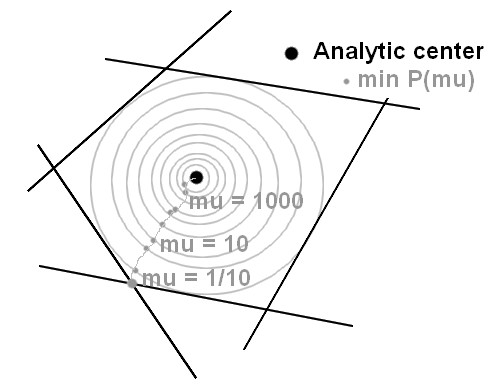
\includegraphics[scale=0.5]{images/12-fig1.jpg} 
\end{center}

\begin{definition} 
\textbf{analytic center:} $x(\infty) = \underset{x\ \in \ \int(X)}{\arg \min} f(x) \qquad (*)$  \\
We call this center "analytic" because it is defined by functions, by calculus. This corresponds to the value of $x$ that minimizes $f(x)$
\end{definition}

\subsection{Barrier Problem} 
We are going tu use the self-concordant function as a barrier to get to the border of the polytope.
\begin{equation}
\label{BarrierProblem}
(p_{\mu}) \qquad \underset{x \in \int X}{\min} \quad \dfrac{c^T x}{\mu} + f(x) = \underset{x \in \int X}{\min} \quad f_{\mu}(x)
\end{equation}
In (\ref{BarrierProblem}) we saw that
\begin{itemize}
\item if $\mu = \infty$, we have the same form than (*), thus, the analytic center is a good approach for the minimum.
\item if $\mu \rightarrow 0$, the point tends to the solution which is on the boundary segment.
\item For every other value of $\mu$, we minimize a balance between the barrier and the objective function
\end{itemize}
As we decrease the value of $\mu$, we get closer to the effective solution of our problem.
\newline
\begin{theorem}
Assuming that $X$ contains no lines, for $\mu > 0$, $x(\mu) = \underset{x \in \int X}{\min} \dfrac{c^T x}{\mu} + f(x)$ is well defined and unique (simply proved)
\end{theorem}
Consider $\lbrace x(\mu) ; \mu > 0 \rbrace$ and call it the \textit{central path}. It tries to be as far as possible from the boundary  and, in the same time, tends to the minimum.\\

\begin{property}
$\underset{\mu \rightarrow 0}{\lim} x(\mu) = x^{\star}$ and it is well defined and optimal for the original problem.
\end{property} 

A possible method would be to target a point $x(\mu)$ and after reaching it jump a bit further on the path and target another point until reaching the true minimum of the objective function. However, this method is too slow (the complexity is not good).\\
So we will introduce a method which will skip some values of $\mu$ but without b too far from the central path.\\
The path is the set of points minimizing $P_\mu$ for different values of $\mu$
\begin{center}
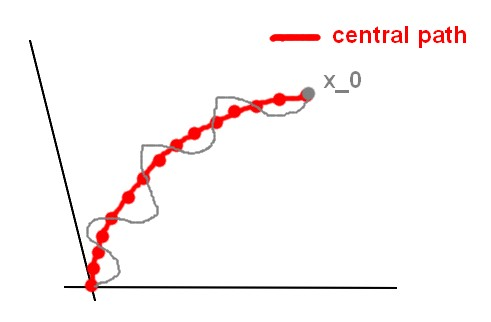
\includegraphics[scale=0.3]{images/12-fig2.jpg} 
\end{center}

\subsection{Proximity measure}
\begin{definition} \textbf{Proximity measure to the central path point $x(\mu)$ :}\\ $$ \delta_{\mu}(x) = || n_{\mu}(x) ||_x $$\\
 with $n_{\mu}(x) = - \nabla^2 f_{\mu}(x)^{-1} \nabla f_{\mu}(x) = - \nabla^2 f(x)^{-1} [\dfrac{c}{\mu} + \nabla f(x)]$\\
\end{definition}

 This corresponds to a Newton step for the min function $f_{\mu}(x)$.\\ Therefore, we successively find
$$\delta_{\mu}(x) = || \nabla f_{\mu}(x) ||_x^{\star} = || \dfrac{c}{\mu} + \nabla f(x) ||_x^{\star}$$
$\delta_{\mu}$ is the space between iter points and central path. Since always requiring to get to the targeted point is too slow, we propose to start from a staring point close to the central path and make only one Newton step per target. The algorithm is the following:\\

\begin{lstlisting}[mathescape,caption=Interior Point Algorithm]
Given $x_0$, $\mu_0$, $0 < \tau < 1$ and $0 < \theta < 1$, such that $\delta_{\mu_0}(x_0) \leq \tau$
While $\mu_k > \mu_{final}$
$\mu_{K+1} = (1 - \theta) \mu_k$ 
$x_{k+1} = x_k + n_{\mu_{k+1}}(x_k)$
$k \leftarrow k + 1$
\end{lstlisting}


\begin{definition} Assume that $f$ is a self-concordant function and $\delta (x) \leq \sqrt{\nu}$ for some $\nu \geq 1$. Then, $f$ is a \textbf{$\nu$-self-concordant barrier}.
\end{definition}

\begin{example}
\begin{leftbar}
$- \log (x)$ is a $1$-self-concordant barrier 
\end{leftbar}
\end{example}

\begin{property}
\textit{if $f_1$ is $\nu_1$-self-concordant barrier, $f_2$ is $\nu_2$-self-concordant barrier then $f_1 + f_2$ is a $(\nu_1 + \nu_2)$-self-concordant barrier}
\end{property}
 
\begin{property}
\textit{$x \rightarrow f(x)$ is $\theta$-self-concordant barrier then $y \rightarrow f(c - A^T y)$ is also $\theta$-self-concordant barrier}
\end{property}

\begin{example}
\begin{leftbar}
Exercices 
\begin{enumerate}
\item $- \log (c_i - a_i^T y)$ is $1$-self-concordant barrier
\item $- \sum_{i=1}^m \log (c_i - a_i^T y)$ is m-self-concordant barrier
\end{enumerate}
\end{leftbar}
\end{example}

Assuming $f$ is a $\nu$-self-concordant barrier. We have $c^T x(\mu) - c^T x^{\star} \leq \nu\mu$.\\
For example, if we have a 6-self-concordant barrier,
\begin{itemize}
\item $x(\frac{1}{10})$ has accuracy $\frac{6}{10}$
\item $x(\frac{1}{1000})$ has accuracy $\frac{6}{1000}$
\end{itemize}
But in practise we never compute $x(\mu)$.\\

\begin{theorem}
Assume $\delta_{\mu}(x) \leq \tau < 1$. Then
$$c^T x(\mu) - c^T x^{\star} < \frac{\nu\mu}{1 - \tau}$$
This means that $\mu_{final}$ is the solution to
$$\frac{\nu\mu}{1 - \tau} = \epsilon$$
\end{theorem}

\subsection{Short-step path following method}

\begin{theorem}
Choosing $\tau = \dfrac{1}{4}$, $\theta = \dfrac{1}{16 \sqrt{\nu}}$, the method 
\begin{enumerate}
\item maintains $\delta_{\mu_k}(x_k) \leq \tau \quad \forall k$ 
\item stops after $\mathcal{O}(\sqrt{\nu} \log(\dfrac{1}{\epsilon}))$ steps
\end{enumerate}
\end{theorem}

This method is known as the \textit{Short-step path following method}. The term $\theta = \dfrac{1}{16 \sqrt{\nu}}$ is too small and the step between two $\mu$ is also too small. Thus, the complexity is too bad.\\

\textbf{How to find $x_0$ and $\mu_0$?}\\
Pick whatever $\mu_0$ you like, depends on the problem (could be heuristic or the central point,...). The chosen $x_0$ must be close to the central path.\\
\textbf{Init:} Pick a reasonable $\mu_0$ and compute $x_0$ by minimization of $(P_{\mu_0}):  \text{min} \dfrac{c^T x}{\mu_0} + f(x)$ using damped Newton steps. Stop the procedure when distance to the path is less or equal to $\dfrac{1}{4}\ (=\tau)$.\\
Let's consider a similar method: long step method.

\subsection{Long step method}

\begin{lstlisting}[mathescape,caption=Long step method]
Given $x_0$, $\mu_0$, $0 < \tau < 1$, $0 < \theta < 1$ such that $\delta_{\mu_0}(x_0) \leq \tau$\\
While $(\mu_k > \mu_{final})$
$\mu_{k+1} = (1 - \theta) \mu_k$ 
Compute $x_{k+1}$ such that $\delta_{\mu_{k+1}}(x_{k+1}) \leq \tau$ $(\star)$
$k \leftarrow k + 1$
End
$(\star)$ using possibly several damped Newton-steps. 
\end{lstlisting}

\begin{theorem}
For any $0 < \tau < 1$ and $0 < \theta < 1$, this method computes a $\nu$-self-concordant barrier and method stops after $O(\nu \log(\dfrac{1}{\epsilon}))$ steps (The number of steps means the number of damped Newton-steps - which is much more than number of $\mu_k$ updates).


\end{theorem}

Remark that this method works good for any $\tau$, $\theta$, which make it flexible. Theoretically, this method is worst than the short step method, but in practice, it rarely needs more than $20$ - $50$ iterations. 

\subsection{Proof that short step method works}

\begin{proof}
\begin{center}
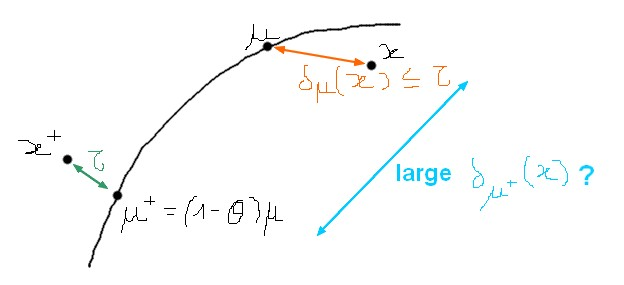
\includegraphics[scale=0.5]{images/12-fig3.jpg} 
\end{center}

Now, $\tau = \dfrac{1}{4}$

\begin{align*}\nonumber
\delta_{\mu_{k+1}}(x_k) &= || \dfrac{c}{\mu_{k+1}} + \nabla f(x_k) ||_{x_k}^{\star} \\ 
\end{align*}
\begin{align*}\nonumber
\text{let} &\quad x_k \rightsquigarrow x\\
&\quad x_{k+1} \rightsquigarrow x^+\\
&\quad \mu_k \rightsquigarrow \mu\\
&\quad \mu_{k+1} \rightsquigarrow \mu^+ = (1-\theta)\mu\\
\end{align*}
\begin{align*}\nonumber
\delta_{\mu_{k+1}}(x_k) &= || \dfrac{c}{\mu^+} + \nabla f(x) ||_x^{\star} \\
& \nonumber = || \dfrac{\mu}{\mu^{+}} (\dfrac{c}{\mu^+} + \nabla f(x)) + (1 - \dfrac{\mu}{\mu^+}) \nabla f(x) ||_x^{\star} \\
& \nonumber \leq \dfrac{1}{1 - \theta} || \dfrac{c}{\mu} + \nabla f(x) ||_x^{\star} + \dfrac{\theta}{1 - \theta} || \nabla f(x) ||_x^{\star} \\
& \nonumber \leq \dfrac{1/4 + 1/(16\sqrt{\nu})  ~ \sqrt{\nu}}{1 - \theta} = \dfrac{5/16}{1 - \theta} \\
& \nonumber \leq \dfrac{5/16}{15/16} = \dfrac{1}{3} \qquad \text{using} \quad \nu \geq 1
\end{align*}
Then $\delta_{\mu^+(x^+)} = \begin{pmatrix}
\dfrac{1/3}{1 - 1/3}
\end{pmatrix}^2 
= \dfrac{1}{4}$
Starting from a point at a distance lower than $\frac{1}{4}$ from the central path, we move forward to another point at a distance lower than $\frac{1}{4}$ from the central path.

\end{proof}

%\end{document}